\documentclass[svgnames,smaller]{beamer}

\usetheme{metropolis}
\usecolortheme{pluritallight}
\metroset{block=fill}

\usepackage[utf8]{inputenc}
\usepackage[T1]{fontenc}
\usepackage{graphicx}
\usepackage{multirow}
\usepackage{tabularx}
\usepackage{booktabs}

\usepackage{geometry}
\geometry{
    left=2.5mm,
    right=2.5mm,
    top=0mm,
    bottom=0mm
}

\usepackage{hyperref}
\usepackage{breakurl}

%===================================================

\definecolor{usnyellow}{RGB}{241, 138, 0}
\definecolor{upnred}{RGB}{226, 6, 19}

\newcommand{\tc}[2]{\textcolor{#1}{#2}}
\renewcommand{\emph}[1]{\textbf{#1}}

\hypersetup{
    colorlinks=true,
    citecolor=orange,
    linkcolor=black,
    urlcolor=blue
}

%===================================================
\title[]{\vspace{3.0em}Programmation et projet encadré - L7TI005}
\subtitle[]{Git : introduction\\%
%\tiny{Crédits supports : Serge Fleury}%
}
\author[shortname]{Yoann Dupont, Serge Fleury \tc{blue}{\tt prenom.nom@sorbonne-nouvelle.fr}\\
Pierre Magistry \href{mailto:pierre.magistry@inalco.fr}{\tt pierre.magistry@inalco.fr}%
}
\institute{Université Sorbonne-Nouvelle\\
INALCO\\
Université Paris-Nanterre\\
%\includegraphics{../common/CC-BY-NC.png}%
}
\date{2022-2023}
\titlegraphic{%
    \vspace{-2.1em}\noindent\makebox[\textwidth]{\includegraphics[width=\paperwidth]{../common/plurital-logo.jpg}}
}

\begin{document}

\begin{frame}
\titlepage
\end{frame}

%===============================================================================

\section{Les bases}

%-------------------------------------------------------------------------------

\begin{frame}{Git et Github}
Git et Github sont deux choses différentes :
\begin{itemize}
    \item Git est un outil créé par Linus Torvald (créateur du noyau Linux)
    \item Github est un service web basé sur Git créé par l'entreprise Github, Inc. (rachetée par Microsoft en 2018)
    \begin{itemize}
        \item Offre un espace de stockage en ligne pour les dépôts Git
        \item Mais aussi d'autres fonctionnalités absentes de Git seul
    \end{itemize}
\end{itemize}
\end{frame}

%-------------------------------------------------------------------------------

\begin{frame}{Git en bref}
\begin{minipage}{0.49\linewidth}
    Git...
    \begin{itemize}[<+->]
        \item ... est un \emph{système de gestion de versions} ou SGV (en anglais \textit{Version Control Software} ou \textit{VCS}).
        \item ... permet de gérer les \emph{modifications} effectuées sur un dossier données de manière \emph{décentralisée}.
        \item ... ne versionne pas des fichiers, mais des ensembles ordonnés de modifications.
    \end{itemize}
\end{minipage}
\begin{minipage}{0.49\linewidth}
    \onslide<4->{
    \begin{figure}
        \centering
        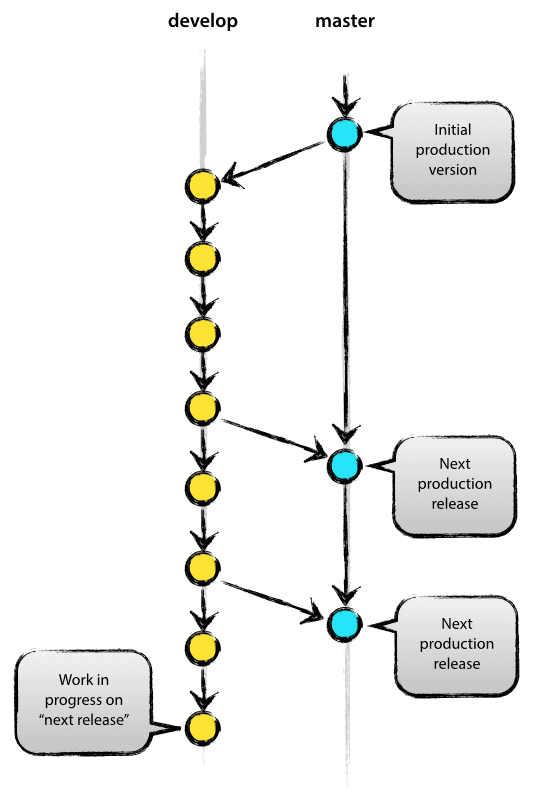
\includegraphics[height=0.75\textheight]{images/main-branches@2x.png}
        \caption{Une vision simplifiée d'un dépôt. À gauche, vos changements locaux, à droite, l'état de votre dépôt distant.}
        % \label{fig:my_label}
    \end{figure}
    }
\end{minipage}
\end{frame}

% %-------------------------------------------------------------------------------

% \begin{frame}{Créer un dépôt GitHub I}
% \begin{figure}
%     \centering
%     \includegraphics[width=0.4\textwidth]{images/gh-new-repo.png}
%     \caption{Une fois connecté·e sur \url{https://github.com}, en haut à droite, cliquez sur "+" puis "new repository".}
%     \label{fig:git_software_manager}
% \end{figure}
% \end{frame}

% %-------------------------------------------------------------------------------

% \begin{frame}{Créer un dépôt GitHub II}
% \begin{minipage}{0.49\linewidth}
%     \begin{itemize}
%         \item \textbf{Repository Name} : PPE1
%         \item \textbf{Description} : Programmation et Projet Encadré 1
%         \item \textbf{Public} : cocher
%         \item \textbf{Add a README file} : cocher
%         \item \textbf{Add a .gitignore} : pas nécessaire ici
%         \item \textbf{Licence} : comme vous voulez
%         \item cliquez sur "create repository"
%     \end{itemize}
% \end{minipage}
% \begin{minipage}{0.49\linewidth}
% \begin{figure}
%     \centering
%     \includegraphics[height=0.9\textheight]{images/gh-new-repo-config.png}
% \end{figure}
% \end{minipage}
% \end{frame}

% %-------------------------------------------------------------------------------

% \begin{frame}{Créer un dépôt GitHub III}
% \begin{center}
%     \large
%     Bravo ! Vous avez à présent votre dépôt git !
    
%     On peut maintenant voir comment on interagit avec.
% \end{center}
% \end{frame}

%===============================================================================

\section{Les commandes git}

%-------------------------------------------------------------------------------

\begin{frame}{Généralités}
Git fournit un ensemble de commandes qui permettent de gérer les changements.

La syntaxe générale prend la forme suivante :
\begin{center}
\large
\texttt{git <sous-commande> [-options...] [arguments...]}
\end{center}

\onslide<2->{
Les commandes git sont paramétrables, on ne traitera ici que des cas de base.

En accord avec la philosophie Unix, les commandes git sont également très précises et font le moins de choses possibles.
}
\end{frame}

%-------------------------------------------------------------------------------

\begin{frame}{git clone}
Permet de créer une copie d'un dépôt existant sur sa machine.

Cette copie peut de suivre et de faire suivre les changements apportés au dépôt. On a donc un \emph{clone} du dépôt distant.

\begin{center}
\large
\texttt{git clone [-options...] <URL>}
\end{center}

Où \texttt{<URL>} est le lien vers un dossier git (généralement distant).

\onslide<2->{
\vfill
\begin{block}{Lier un dépôt de travail à son compte GitHub}
En supposant que \texttt{USER} soit votre identifiant GitHub et \texttt{EMAIL} votre email :

\texttt{git config user.name "USER"} \\
\texttt{git config user.email "EMAIL"}

On peut mettre l'option \texttt{--global} pour ne pas faire ces deux lignes à chaque fois.
\end{block}
}
\end{frame}

%-------------------------------------------------------------------------------

\begin{frame}{git pull}
Permet de mettre-à-jour votre branche vers la bonne version (par défaut : la dernière version en ligne).

En termes git, on \emph{tire} les changements du dépôt distant vers notre répertoire local.
\begin{center}
\large
\texttt{git pull}
\end{center}
\end{frame}

%-------------------------------------------------------------------------------

\begin{frame}{git add}
Permet d'indiquer des fichiers dont on veut suivre les modifications avant validation.

En terminologie git, on \emph{ajoute au suivi} des modifications faites sur des fichiers. On appelle cette étape la mise-en-place (\textit{staging}).

\begin{center}
\large
\texttt{git add <FILE...>}
\end{center}

Où \texttt{<FILE...>} est un ou plusieurs fichiers dont on souhaite suivre les modifications

\onslide<2->{
    \vfill
    \begin{alertblock}{\textbf{Attention :}}
    \texttt{git add} suit les modifications \emph{passées, mais pas futures}. Si vous modifiez un fichiers après un \texttt{add}, ces nouveaux changements ne seront pas suivis.
    \end{alertblock}
}
\end{frame}

%-------------------------------------------------------------------------------

\begin{frame}{git commit}
Permet de valider les modifications des fichiers suivis.

Pourquoi \textit{commit} ? De nouvelles modifications peuvent être faites après un commit, mais git \emph{se tiendra} aux modifications validées.

\begin{center}
\large
\texttt{git commit [-m message]}
\end{center}

Où \texttt{message} est le message qui décrit les changements que vous faites.

\onslide<2->{
    \vfill
    \begin{alertblock}{\textbf{Attention :}}
    Si aucun message n'est donné, git ouvrira un éditeur de texte dans le terminal pour que vous puissiez écrire. Ça peut faire de mauvaises surprises.
    \end{alertblock}
}
\end{frame}

%-------------------------------------------------------------------------------

\begin{frame}{git push}
\textbf{Envoie} les modifications mises en place (ou "commitées") vers le dépôt distant.

On dit, en git, qu'on \textbf{pousse} les modifications.

\begin{center}
\large
\texttt{git push}
\end{center}
\end{frame}

%-------------------------------------------------------------------------------

\begin{frame}{git status}
Permet de voir les changements de votre dossier par rapport à la version du dépôt.
\begin{center}
\large
\texttt{git status}
\end{center}

Cela affichera les fichiers mis en place (\textit{staged}) et les modifications non suivies.
\end{frame}

%-------------------------------------------------------------------------------

\begin{frame}[standout]
Et maintenant la pratique
\end{frame}

%-------------------------------------------------------------------------------

\begin{frame}{Installer git}
\begin{figure}
    \centering
    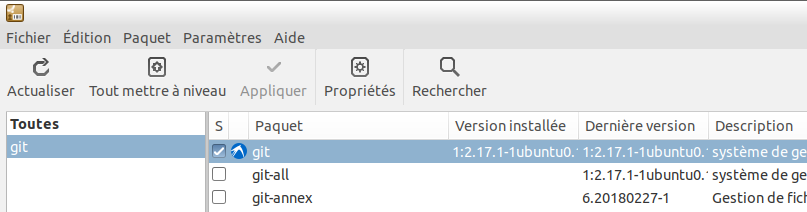
\includegraphics[width=0.9\textwidth]{images/git-software-manager.png}
    \caption{Allez dans le logiciel de gestion des programmes et sélectionnez tout simplement "git" pour installation.}
    \label{fig:git_software_manager}
\end{figure}
\end{frame}

%-------------------------------------------------------------------------------

\begin{frame}{git clone - Premier test}
\begin{exampleblock}{Petit test - récupérer les slides du cours}
Créez-vous un dossier plurital quelque part \textbf{PAS SUR LE BUREAU}.

Allez dedans et tapez la commande suivante :

\texttt{git clone https://github.com/YoannDupont/PPE.git}

Inutile de lier vos identifiants à ce compte, vous ne pourrez pas pousser.
\end{exampleblock}
\end{frame}

%-------------------------------------------------------------------------------

\end{document}
